\section{Resultados}
En esta sección se muestran las secciones transversales para elipsoides oblatos, empleados como una primera aproximación a la forma discoide cóncava de los eritrocitos. Dado que los eritrocitos en una muestra real no interactúan fuertemente entre ellos \footnote{poner pie de página mencionando que son medio transparentes o que hacen poco contaste con el agua} y que se encuentran orientados de forma aleatoria, es posible estudiar su respuesta óptica considerando una sola partícula y definir una respuesta promedio en términos de las secciones transversales promedio $\langle C_{ext} \rangle$, $\langle C_{abs} \rangle$ y $\langle C_{sca} \rangle$. Con estas cantidades, se considera que una onda plana puede excitar de forma eficiente el sistema en sus tres ejes de forma homogénea. \footnote{Considerando que las partículas no sean ópticamente activas.} Estas están dadas por \cite{Bohren}:
\begin{align*}
	\langle C_{abs}\rangle &= \frac{k}{3} \text{Im}\{\alpha^{(1)}+\alpha^{(2)}+\alpha^{(3)}\},\\
	\langle C_{sca}\rangle &= \frac{k^4}{3(6\pi)} \left(\alpha^{(1)}+\alpha^{(2)}+\alpha^{(3)}\right)^2.
\end{align*}

Para caracterizar la respuesta dieléctrica del material, se emplea la función dieléctrica $\epsilon(\omega)$, la cual puede determinarse experimentalmente a partir del índice de refracción complejo de un medio, $\tilde{n}(\omega) = n(\omega) + i\kappa(\omega)$. La relación entre la función dieléctrica y el índice de refracción está dada por las expresiones \cite{Plasmonics}
\begin{align} 
	\text{Re}[\epsilon(\omega)] &= n^2 - \kappa^2,\\
	\text{Im}[\epsilon(\omega)] &= 2n\kappa, \end{align}
donde $\kappa$ es el coeficiente de extinción, el cual describe la absorción de las ondas electromagnéticas al propagarse en el medio \cite{Plasmonics}.\\

Debido a su dependencia exclusiva de la frecuencia, es conveniente expresar a la función dieléctrica mediante el modelo de Drude, pues ofrece un mayor control sobre la respuesta óptica del sistema, resultando adecuado para estudiar la respuesta general y familiarizarse con el sistema. El modelo de Drude es particularmente útil para describir el comportamiento plasmónico de materiales a frecuencias bajas y en los que la respuesta óptica está dominada por electrones libres, como en los metales, donde los electrones en la banda de conducción responden colectivamente a un campo electromagnético aplicado. Mediante este modelo, se expresa a la función dieléctrica como \cite{Plasmonics}
\begin{equation} \epsilon(\omega) = 1 - \frac{\omega_p^2}{\omega^2 + i\gamma\omega}, \end{equation}
donde $\omega_p$ es la frecuencia de plasma del material y $\gamma$ es la constante fenomenológica de amortiguamiento. \\

Para analizar las contribuciones de las secciones transversales en partículas elipsoidales oblatas dentro del régimen cuasiestático, en la Fig. \ref{Contribuciones} se muestran las $\langle C_{ext} \rangle$ (línea azul), $\langle C_{sca} \rangle$(línea verde) y $\langle C_{abs} \rangle$ (línea roja). Estas cantidades se grafican en escala logarítmica en función de $\lambda$ (eje superior) y $\hbar\omega$ (eje inferior) de la onda electromagnética incidente. Las partículas elipsoidales oblatas son modeladas con una función dieléctrica dada por el modelo Drude, cuyos parámetros son $\hbar\omega_p=13.142\text{ eV}$ y $\hbar\gamma=0.197\text{ eV}$. Sus semiejes están dados por $a=1.5\text{ nm}$, $c=1\text{ nm}$ y se encuentra inmersa en una matriz con índice de refracción $n_m=1.33$. \\
\begin{figure}[h!]
	\sidesubfloat[]{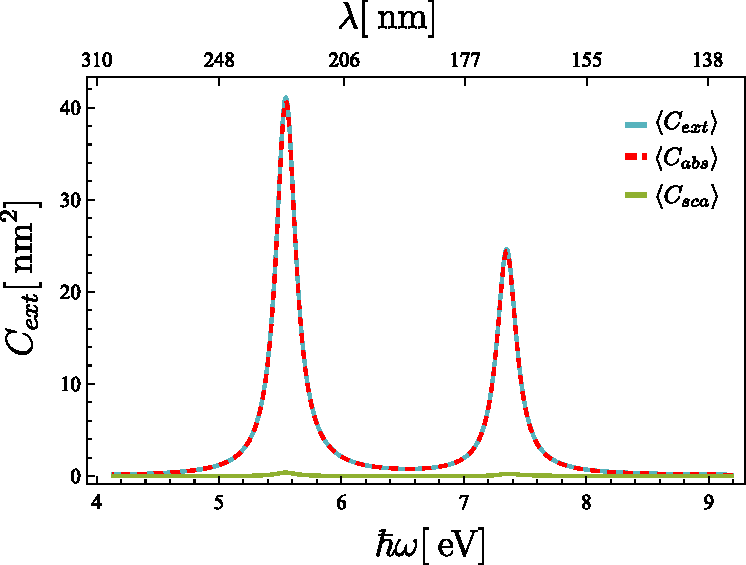
\includegraphics[width=.445\textwidth]{../../Figuras/AlContribuciones3.pdf} \label{Contribuciones}}\quad%
	\sidesubfloat[]{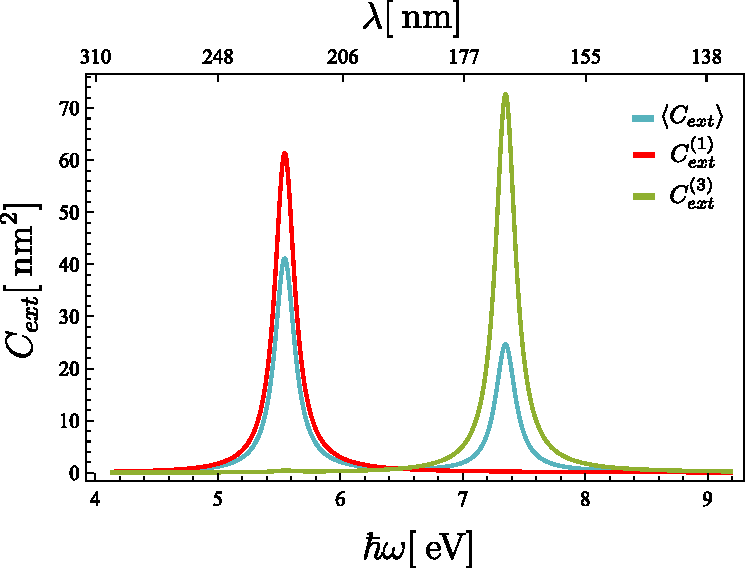
\includegraphics[width=.44\textwidth]{../../Figuras/CextAlbueno.pdf}\label{Cextpromedio}}%
	\caption{Secciones transversales como función de la energía $\hbar\omega$ y de la longitud de onda $\lambda$ para una partícula elipsoidal oblata de aluminio caracterizada por su función dieléctrica dada por el modelo de Drude ($\hbar\omega_p=13.142\text{ eV}$, $\hbar\gamma=0.197\text{ eV}$), con semiejes $a=b=1.5\text{ nm}$, $c=1\text{ nm}$ e inmersa en un medio acuoso ($n_m=1.33$). \textbf{a)}  Sección transversal de extinción promedio $\langle C_{ext}\rangle$  (línea azul), sección transversal de absorción promedio $\langle C_{abs}\rangle$  (línea roja) y sección transversal de esparcimiento promedio $\langle C_{sca}\rangle$  (línea verde) en escala logarítmica. \textbf{b)} Sección transversal de extinción promedio $\langle C_{ext}\rangle$ (línea azul), sección transversal de extinción al iluminar a la partícula con una onda polarizada en la dirección $\hat{e}_x$, $C_{ext}^{(1)}$  (línea roja)  y sección transversal de extinción al iluminar la partícula con una onda polarizada en la dirección $\hat{e}_z$ $C_{ext}^{(3)}$  (línea verde).} \label{fig:test}
\end{figure}

A partir de los resultados mostrados en la Fig. \ref{Contribuciones}, se observa que, en partículas dentro del régimen cuasiestático, la absorción domina sobre el esparcimiento en la contribución a la extinción. Esto se evidencia en la diferencia de magnitudes entre ambas curvas, donde la absorción es aproximadamente tres órdenes de magnitud mayor que el esparcimiento y la curva de extinción es escencialmente la misma que la de absorción. Debido a esta marcada diferencia, los análisis posteriores se enfocan exclusivamente en las secciones transversales de extinción, ya que el impacto del esparcimiento es despreciable.\\

El análisis de las diferencias entre la $\langle C_{ext}\rangle$ y aquellas obtenidas al iluminar la partícula con una onda polarizada en una única dirección se presenta en la Fig. \ref{Cextpromedio}. En esta figura se muestran las $\langle C_{ext}\rangle$ (línea azul), $C_{ext}^{(1)}$ y $C_{ext}^{(3)}$ (línea verde). Estos cálculos corresponden a un sistema con las mismas características que el de la Fig. \ref{Contribuciones}.\\

En la Fig. \ref{Cextpromedio} se observa que debido a la geometría de la partícula, que es un elipsoide oblato, la 
$\langle C_{ext}\rangle$ presenta dos máximos, los cuales coinciden con las frecuencias de los máximos de $C_{ext}^{(1)}$ y $C_{ext}^{(3)}$. Esto muestra que las secciones transversales promedio son útiles para representar el efecto de iluminar una partícula elipsoidal con una onda electromagnética polarizada en la dirección de cualquiera de sus tres ejes principales, ya que lo que cambia es la amplitud de los máximos en la sección transversal promedio más no la localización espectral de estos. \\

Las siguientes figuras presentan los cálculos de las secciones tranversales de extinción promedio  $\langle C_{ext}\rangle$ considerando nanopartículas elipsoidales oblatas cuya función dieléctrica está caracterizada por el modelo de Drude para aluminio \cite{Aluminio} y por datos experimentales para plata \cite{Plata}, oro \cite{Plata}, bismuto \cite{Bismuto} y  óxido de magnesio \cite{MgO}.


\subsection*{Aluminio y plata}
En la Fig. \ref{aluminioplataAR} se muestran las $\langle C_{ext}\rangle$ en función de $\hbar\omega$ (eje inferior) y de  $\lambda$ (eje superior) de la onda electromagnética incidente en nanopartículas elipsoidales oblatas de aluminio (AlNPs) (Fig. \ref{aluminioAR}) y plata (AgNPs) (Fig. \ref{plataAR}). La función dieléctrica para las AgNPs está dada por el modelo de Drude con parámetros $\hbar\omega_p=13.142\text{ eV}$, $\hbar\gamma=0.197\text{ eV}$, mientras que para las AlNPs  está dada por datos experimentales obtenidos de \cite{Plata}. Se realizan los cálculos para partículas elipsoidales con razón de aspecto AR=2 y con semiejes de tamaños desde 1 nm a 2.5 nm, en pasos de 0.5 nm; cada caso se identifica con el código de color mostrado en la gráfica. Asimismo, se realizan los cálculos para una partícula esférica con $a2 \text{ nm}$ (línea gris punteada) con relación de aspecto AR$=1$. Todas las partículas se consideran inmersas en un medio acuoso con $n_m=1.33$.\\

\begin{figure}[h!]
	\sidesubfloat[]{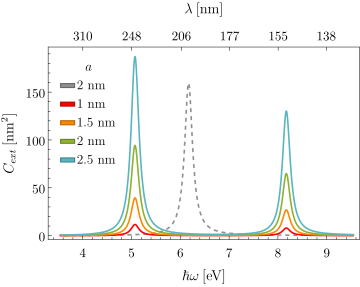
\includegraphics[width=.445\textwidth]{../../Figuras/AlAR} \label{aluminioAR}}\quad%
	\sidesubfloat[]{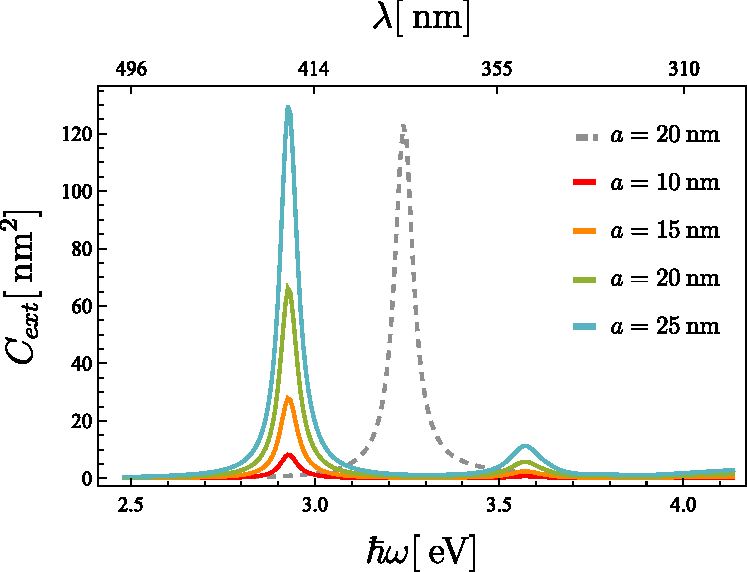
\includegraphics[width=.44\textwidth]{../../Figuras/AgAR}\label{plataAR}}%
	\caption{Secciones transversales de extinción promedio $\langle C_{ext}\rangle$ como función de la energía $\hbar\omega$ y de la longitud de onda $\lambda$ de la onda electromagnética incidente para una partícula elipsoidal oblata con razón de aspecto $AR=a/c=2$ constante, excepto en el caso de una esfera (línea gris punteada) donde $AR=1$. Las partículas poseen semiejes de tamaños $a=2.5 \text{ nm}, c=1.25 \text{ nm}$ (línea azul), $a=2 \text{ nm}, c=1 \text{ nm}$ (línea verde), $a=1.5 \text{ nm}, c=0.75 \text{ nm}$ (línea naranja), $a=1 \text{ nm}, c=0.5 \text{ nm}$ (línea roja) y $a=b=c=2\text{ nm}$ (línea gris punteada). Las partículas se encuentran inmersas en un medio acuoso ($n_m=1.33$) y están caracterizadas por su función dieléctrica dada por  \textbf{a)} el modelo de Drude para el aluminio con parámetros $\hbar\omega_p=13.142\text{ eV}$ y $\hbar\gamma=0.197\text{ eV}$) y \textbf{b)} datos experimentales correspondientes a la plata obtenidos de \cite{Plata}. }\label{aluminioplataAR}
\end{figure}
A partir de los resultados de la Fig. \ref{aluminioplataAR}, se observa que al aumentar el tamaño de la partícula mientras se mantiene constante AR, la localización espectral de las resonancias no cambia pero que su valor nominal aumenta. Se identifican dos máximos locales en $\langle C_{ext}\rangle$,  los cuales corresponden a las frecuencias en las que $C_{ext}^{(1)}$ y $C_{ext}^{(3)}$ se maximizan. Para $C_{ext}^{(1)}$, las resonancias  se encuentran en $\lambda=$254 nm para el aluminio y $\lambda=$434 nm para la plata. Para $C_{ext}^{(3)}$, las resonancias ocurren en $\lambda=$146 nm para aluminio y $\lambda=$344 nm para la plata. \\

El efecto de la variación de la relación de aspecto en la sección transversal de extinción promedio en partículas de aluminio y plata inmersas en un medio acuoso ($n_m=1.33$) se muestra en la Fig. \ref{aluminioplatac}. Se muestra la $\langle C_{ext}\rangle$ en función de $\hbar\omega$ y de $\lambda$  de la onda electromagnética incidente en AgNPs (Fig. \ref{aluminioc}) y AlNPs (Fig. \ref{platac}). Las funciones dieléctricas utilizadas para las partículas de aluminio y las de plata son las mismas que en la Fig. \ref{aluminioplataAR}. Se grafica para partículas elipsoidales con razones de aspecto desde 1.5 a 2.25, en pasos de 0.25 y con $c=1\text{ nm}$. Asimismo, se realizan los cálculos para una partícula esférica con  $c=1\text{ nm}$ y con razón de aspecto AR$=1$. 


\begin{figure}[h!]
	\sidesubfloat[]{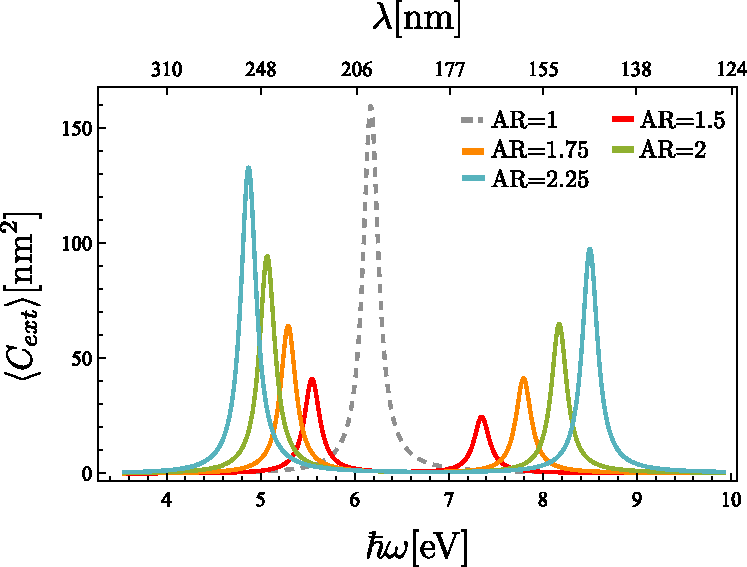
\includegraphics[width=.445\textwidth]{../../Figuras/Alc} \label{aluminioc}}\quad%
	\sidesubfloat[]{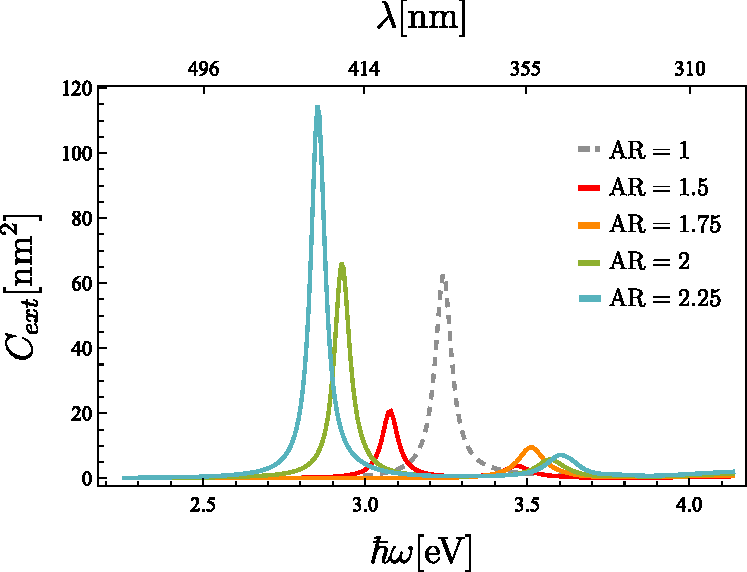
\includegraphics[width=.44\textwidth]{../../Figuras/Agc}\label{platac}}%
	\caption{Secciones transversales de extinción promedio $\langle C_{ext}\rangle$ como función de la energía $\hbar\omega$ y de la longitud de onda $\lambda$ de la onda electromagnética incidente para una partícula elipsoidal oblata y una esférica. Las partículas elipsoidales poseen un semieje menor de tamaño $c=1nm$ y presentan razones de aspecto de AR=1.5 (línea roja), AR=1.75 (línea naranja), AR=2 (línea verde), AR=2.25 (línea azul), mientras que la esférica tiene una razón de aspecto AR=1 (línea gris punteada). Las partículas están inmersas en un medio acuoso ($n_m=1.33$) y están caracterizadas por su función dieléctrica dada por  \textbf{a)} el modelo de Drude para el aluminio ($\hbar\omega_p=13.142\text{ eV}$, $\hbar\gamma=0.197\text{ eV}$) y \textbf{b)} datos experimentales correspondientes a la plata obtenidos de \cite{Plata}.}\label{aluminioplatac}
\end{figure} 

 En las Figs. \ref{aluminioc}  y \ref{platac} se observa que conforme la relación de aspecto se aproxima a la unidad, hay un corrimiento de las frecuencias asociadas a las $\langle C_{ext}\rangle$ máximas hacia la frecuencia de resonancia asociada a una partícula esférica. Esta frecuencia de resonancia corresponde a $\lambda=201\text{ nm}$ para el aluminio y $\lambda=383\text{ nm}$ para la plata. Además, tanto en el aluminio como en la plata, se observa que al aumentar la relación de aspecto y la longitud del eje mayor, la amplitud de  $\langle C_{ext}\rangle$ también aumenta. Esto se debe a que una mayor sección transversal efectiva de interacción con la onda electromagnética incrementa la probabilidad de esparcimiento y absorción de luz, lo que, en consecuencia, aumenta la extinción.



\subsection*{Oro y bismuto}
De forma análoga a el análisis en la variación parámetros geométricos de las NPs rlipsoidales modeladas por Drude, se muestra en la Fig. \ref{oro} la respuesta óptica variando estos parámetros (semieje mayor y razón de aspecto) considerando ahora una función dieléctrica de un material real. En particular, en Fig. 10a) se grafica Cext como función de la energía (eje ingferior) y de la longitud de onda (eje superior() para nanopartículas elipsoidales oblatas de oro (AuNPs) de distintos tamaños que conservan la razón de aspecto de AR=2; para complementar el análisis, se muestra debajo de esta gráfica la función dieléctrica del oro con los datos obtenidos de \cite{Plata}. En la Fig. \ref{oroAR} se consideran partículas con relación de aspecto AR$=2$ con radios desde 1  nma 2.5 nm, en pasos de 0.5 nm; cada caso se identifica con el codig de color mistrado en la gráfica respecticva. También se considera una partícula con relación de aspecto AR$=1$ y semiejes $a=b=c=2$ nm (línea gris), que representa a una partícula esférica. Por otro lado, en la Fig. \ref{oroc} se consideraron partículas con relación de aspecto variable AR=1.5 (línea roja), AR=1.75 (línea naranja), AR=2 (línea verde) y AR=2.25 (línea azul) que presentan valores en su semieje menor $c=1\text{ nm}$. Asimismo, se considera una partícula esférica con semieje mejor $c=1\text{ nm}$ y con relación de aspecto AR$=1$ (línea gris).
\begin{figure}[H]
	\sidesubfloat[]{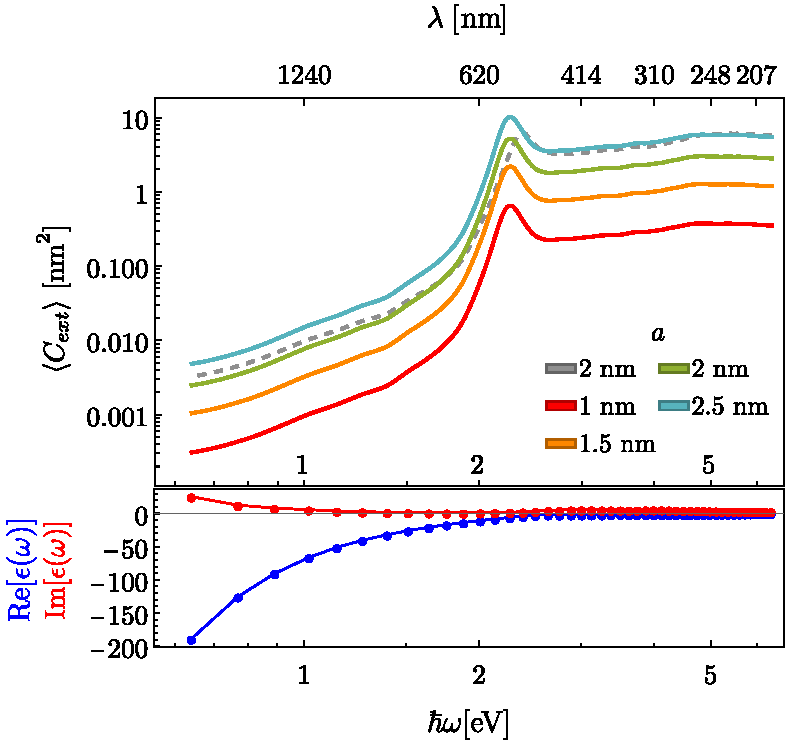
\includegraphics[width=.445\textwidth]{../../Figuras/Au2.pdf} \label{oroAR}}\quad%
	\sidesubfloat[]{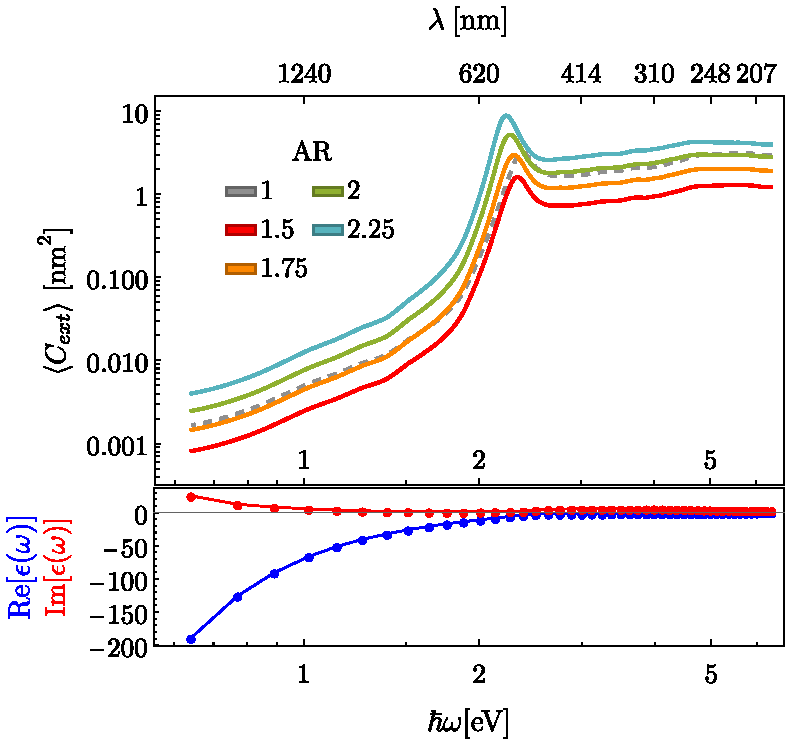
\includegraphics[width=.44\textwidth]{../../Figuras/Au.pdf}\label{oroc}}%
	\caption{Secciones transversales de extinción promedio $\langle C_{ext}\rangle$ como función de la energía $\hbar\omega$ y de la longitud de onda $\lambda$ para una partícula elipsoidal oblata de oro, cuyo índice de refracción complejo fue obtenido a partir de datos experimentales  e inmersa en agua ($n_m=1.33$) y curvas de comparación del índice de refracción (parte real en azul, parte imaginaria en rojo) como función de la energía $\hbar\omega$ y de la longitud de onda $\lambda$ para el oro. \textbf{a)} Razón de aspecto $AR=2$ constante, excepto en el caso de una esfera (línea gris punteada) donde $AR=1$. \textbf{b)} Semieje menor $c=1$ nm constante.}\label{oro}
\end{figure}

En contraste con el aluminio y la plata, en la Fig. \ref{oro} se observa solo una frecuencia de resonancia en $\lambda=$ 547 nm, que se atribuye a la fuerte absorción del oro en el espectro visible, lo que suprime resonancias adicionales. El aumento de la sección transversal de extinción se debe a que para energías mayores a 1.76 eV, los electrones ligados empiezan a contribuir significativamente por medio de transiciones interbanda. Se observa que conforme la relación de aspecto se aproxima a la unidad, hay un corrimiento de las frecuencias asociadas a las $\langle C_{ext}\rangle$ máximas hacia una frecuencia de resonancia ($557\text{ nm}$) asociada a una esfera de oro inmersa en agua. 



En la Fig. \ref{bismuto} se observan las secciones transversales de extinción promedio para partículas de bismuto, así como la parte imaginaria y real de su índice de refracción. En la Fig. \ref{bismutoAR} se consideraron partículas con relación de aspecto AR$=2$  y en la Fig. \ref{bismutoc} se consideraron partículas con relación de aspecto variable. En ambas figuras es posible observar una frecuencia de resonancia de alrededor de los 154 nm.

\begin{figure}[H]
	\sidesubfloat[]{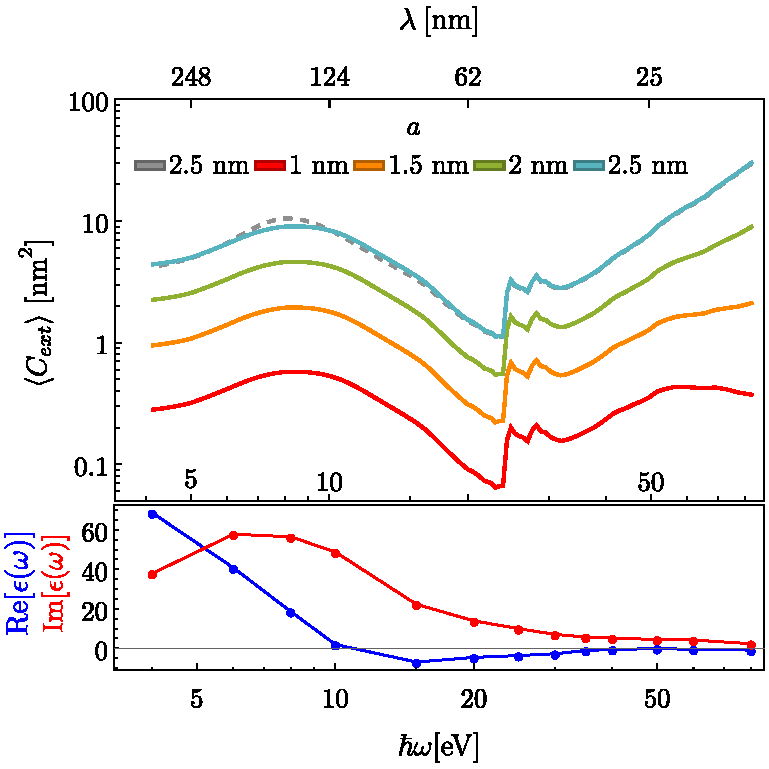
\includegraphics[width=.445\textwidth]{../../Figuras/Bi2} \label{bismutoAR}}\quad%
	\sidesubfloat[]{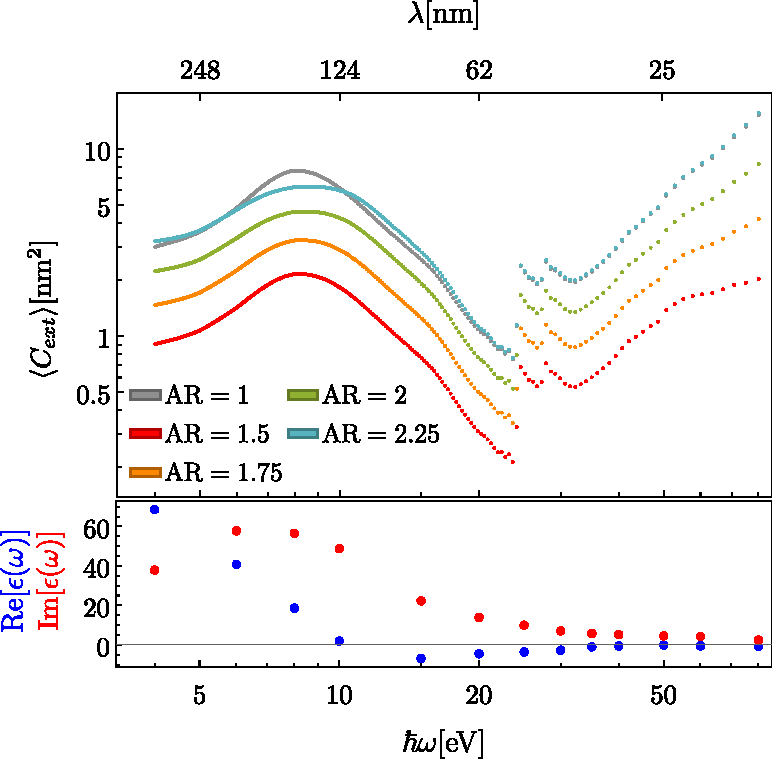
\includegraphics[width=.44\textwidth]{../../Figuras/Bi}\label{bismutoc}}%
	\caption{Secciones transversales de extinción promedio $\langle C_{ext}\rangle$ como función de la energía $\hbar\omega$ y de la longitud de onda $\lambda$ para una partícula elipsoidal oblata de bismuto, cuyo índice de refracción complejo fue obtenido a partir de datos experimentales  e inmersa en agua ($n_m=1.33$) y curvas de comparación de la función dieléctrica (parte real en azul, parte imaginaria en rojo) como función de la energía $\hbar\omega$ y de la longitud de onda $\lambda$ para el bismuto. \textbf{a)} Razón de aspecto $AR=2$ constante, excepto en el caso de una esfera (línea gris punteada) donde $AR=1$. \textbf{b)} Semieje menor $c=1$ nm constante.}\label{bismuto}
\end{figure}


\subsection*{Óxido de magnesio}
En la Fig. \ref{mgo} se observan las secciones transversales de extinción promedio para partículas de bismuto, así como la parte imaginaria y real de su índice de refracción. En la Fig. \ref{mgoAR} se consideraron partículas con relación de aspecto AR$=2$  y en la Fig. \ref{mgoc} se consideraron partículas con relación de aspecto variable. En ambos casos se observa que la $\langle C_{ext}\rangle$ tiene un comportamiento creciente pues, dado que en el espectro de las ondas de radio, la contribución de la absorción es nula y la única contribución es la del esparcimiento, que aumenta al disminuir la longitud de onda.

\begin{figure}[H]
	\sidesubfloat[]{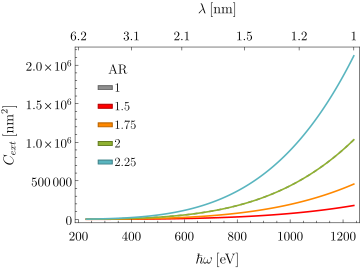
\includegraphics[width=.445\textwidth]{../../Figuras/MgOc} \label{mgoc}}\quad%
	\sidesubfloat[]{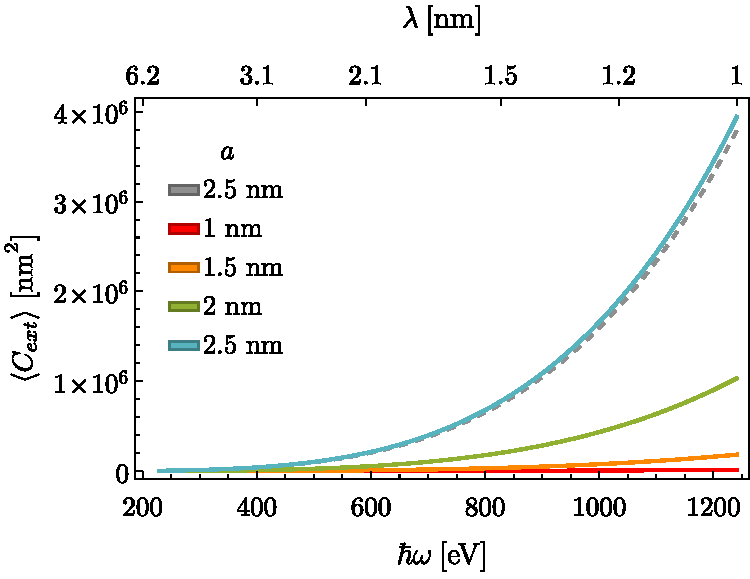
\includegraphics[width=.44\textwidth]{../../Figuras/MgOAR}\label{mgoAR}}%
	\caption{Secciones transversales de extinción promedio $\langle C_{ext}\rangle$ como función de la energía $\hbar\omega$ y de la longitud de onda $\lambda$ para una partícula elipsoidal oblata de óxido de magnesio, cuyo índice de refracción complejo fue obtenido a partir de datos experimentales  e inmersa en agua ($n_m=1.33$) y curvas de comparación de la función dieléctrica (parte real en azul, parte imaginaria en rojo) como función de la energía $\hbar\omega$ y de la longitud de onda $\lambda$ para el bismuto. \textbf{a)} Razón de aspecto $AR=2$ constante, excepto en el caso de una esfera (línea gris punteada) donde $AR=1$. \textbf{b)} Semieje menor $c=1$ nm constante.}\label{mgo}
\end{figure}

Tiene transiciones interbanda a energías muy bajas (~0.15 - 0.2 eV, en el infrarrojo medio).
Se comporta como un semimetal, con una densidad de estados electrónica muy baja en el nivel de Fermi.
En el visible y el infrarrojo cercano, su respuesta óptica es más compleja y no sigue el modelo simple de plasma.







